\documentclass[12pt,letterpaper]{article}

% Packages
\usepackage[margin=1in]{geometry}
\usepackage{graphicx}
\usepackage{amsmath}
\usepackage{booktabs}
\usepackage{listings}
\usepackage{xcolor}
\usepackage{float}
\usepackage{hyperref}
\usepackage{caption}
\usepackage{array}

% Code listing style
\lstset{
    language=[Sharp]C,
    basicstyle=\ttfamily\small,
    keywordstyle=\color{blue}\bfseries,
    commentstyle=\color{green!60!black}\itshape,
    stringstyle=\color{red},
    numbers=left,
    numberstyle=\tiny\color{gray},
    stepnumber=1,
    numbersep=8pt,
    backgroundcolor=\color{gray!10},
    showspaces=false,
    showstringspaces=false,
    showtabs=false,
    frame=single,
    tabsize=4,
    captionpos=b,
    breaklines=true,
    breakatwhitespace=false,
    xleftmargin=2em,
    xrightmargin=2em
}

% Hyperref setup
\hypersetup{
    colorlinks=true,
    linkcolor=blue,
    filecolor=magenta,
    urlcolor=cyan,
    pdftitle={CPU Scheduling Simulator - Performance Analysis},
    pdfauthor={Jack Vega}
}

% Title page information
\title{
    \textbf{CPU Scheduling Simulator}\\
    \large Performance Analysis and Algorithm Comparison\\
    \vspace{1cm}
    Project 2
}
\author{
    Jack Vega\\
    CS 3502: Operating Systems\\
    Kennesaw State University
}
\date{\today}

\begin{document}

\maketitle
\newpage

\tableofcontents
\newpage

% ============================================================
% SECTION 1: INTRODUCTION
% ============================================================
\section{Introduction}

For this project, I extended the provided CPU scheduling simulator by adding 
two new scheduling algorithms: Shortest Remaining Time First (SRTF) and 
Highest Response Ratio Next (HRRN). The main goal was to compare how different 
CPU scheduling algorithms perform under various workload conditions.

\subsection{Project Overview}

The starter code already had FCFS, SJF, Priority, and Round Robin implemented. 
My task was to add:

\begin{itemize}
    \item Two new scheduling algorithms (SRTF and HRRN)
    \item Additional performance metrics like CPU Utilization and Throughput
    \item A CSV export feature to make analyzing the results easier
\end{itemize}

\subsection{What I'm Testing}

The main objectives for this project were:

\begin{enumerate}
    \item Get SRTF (preemptive) and HRRN (non-preemptive) working correctly
    \item Calculate detailed performance metrics for all six algorithms
    \item Compare how each algorithm performs with different types of workloads
    \item Figure out which algorithms work best for different scenarios
\end{enumerate}

\newpage

% ============================================================
% SECTION 2: TECHNICAL IMPLEMENTATION
% ============================================================
\section{Implementation Details}

\subsection{Algorithm 1: Shortest Remaining Time First (SRTF)}

\subsubsection{How SRTF Works}

SRTF is basically a preemptive version of SJF. At each time unit, the scheduler 
looks at all the processes that have arrived and picks the one with the shortest 
remaining burst time. If a new process shows up with a shorter remaining time 
than what's currently running, it preempts (interrupts) the current process.

The main characteristics are:
\begin{itemize}
    \item \textbf{Type}: Preemptive
    \item \textbf{Selection}: Always chooses the process with minimum remaining time
    \item \textbf{Advantage}: Usually gives the best average waiting time
    \item \textbf{Disadvantage}: Long processes can get starved if short ones keep arriving
\end{itemize}

\subsubsection{My Implementation}

I implemented SRTF by keeping track of how much time each process has left and 
checking at every time unit to see if there's a better choice:

\begin{lstlisting}[caption={SRTF Implementation}]
private List<SchedulingResult> RunSRTFAlgorithm(
    List<ProcessData> processes)
{
    var remainingTimes = new Dictionary<string, int>();
    var startTimes = new Dictionary<string, int>();
    var completionTimes = new Dictionary<string, int>();
    
    // Initialize remaining times
    foreach (var process in processes)
    {
        remainingTimes[process.ProcessID] = process.BurstTime;
        startTimes[process.ProcessID] = -1;
    }
    
    int currentTime = 0;
    int completed = 0;
    
    while (completed < processes.Count)
    {
        // Find available processes
        var availableProcesses = processes
            .Where(p => p.ArrivalTime <= currentTime &&
                        remainingTimes[p.ProcessID] > 0)
            .OrderBy(p => remainingTimes[p.ProcessID])
            .ThenBy(p => p.ArrivalTime)
            .ToList();
        
        if (availableProcesses.Count == 0)
        {
            // Jump to next arrival
            currentTime = processes
                .Where(p => remainingTimes[p.ProcessID] > 0)
                .Min(p => p.ArrivalTime);
            continue;
        }
        
        var selectedProcess = availableProcesses.First();
        
        // Record start time if first execution
        if (startTimes[selectedProcess.ProcessID] == -1)
        {
            startTimes[selectedProcess.ProcessID] = currentTime;
        }
        
        // Execute for 1 time unit
        remainingTimes[selectedProcess.ProcessID]--;
        currentTime++;
        
        // Check completion
        if (remainingTimes[selectedProcess.ProcessID] == 0)
        {
            completed++;
            completionTimes[selectedProcess.ProcessID] = currentTime;
        }
    }
    
    // Calculate metrics and return results
    return results;
}
\end{lstlisting}

\subsubsection{Algorithm Steps}

Here's the basic logic in pseudocode form:

\begin{verbatim}
Algorithm: SRTF

1. Initialize remaining_times[] = burst_times[] for all processes
2. Set current_time = 0, completed = 0

3. While completed < total_processes:
   a. Find processes where arrival_time <= current_time
   b. If no processes available:
      - Advance current_time to next arrival
   c. Select process with minimum remaining_time
   d. Execute for 1 time unit
   e. Decrement remaining_time
   f. If remaining_time == 0:
      - Mark as completed
      - Calculate metrics
      
4. Return results
\end{verbatim}

% Placeholder for SRTF screenshot
\begin{figure}[H]
    \centering
    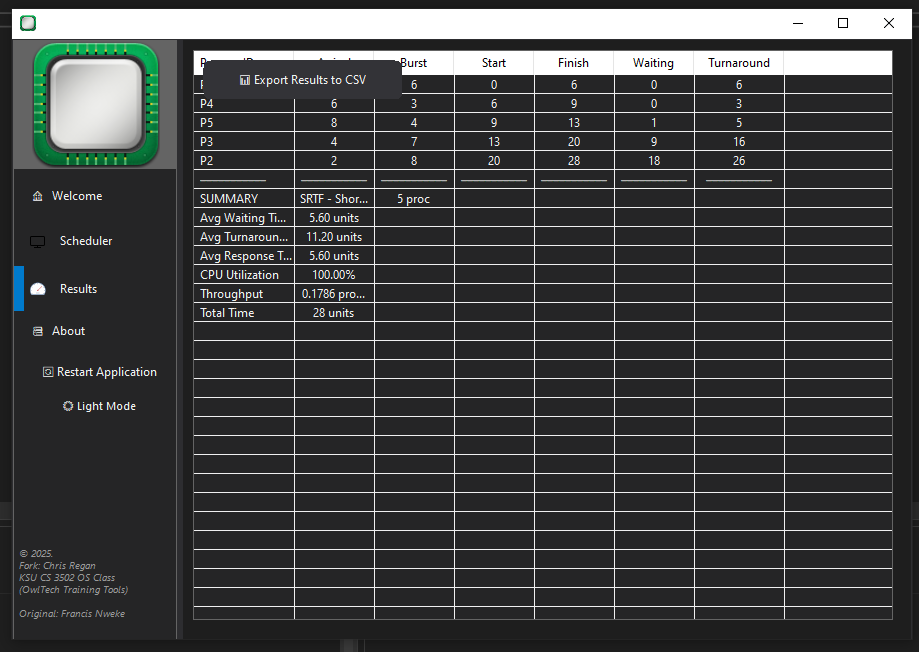
\includegraphics[width=0.9\textwidth]{srtf_results.png}
    \caption{SRTF Algorithm Results}
    \label{fig:srtf}
\end{figure}

\newpage

\subsection{Algorithm 2: Highest Response Ratio Next (HRRN)}

\subsubsection{How HRRN Works}

HRRN is designed to fix the starvation problem in SJF by taking both burst time 
and waiting time into account. It calculates a "response ratio" for each waiting 
process and picks the one with the highest ratio. The formula is:

\[
\text{Response Ratio} = \frac{\text{Waiting Time} + \text{Burst Time}}{\text{Burst Time}}
\]

This is pretty clever because as a process waits longer, its ratio goes up, so 
it eventually gets chosen even if it has a long burst time. This prevents any 
process from waiting forever.

Key features:
\begin{itemize}
    \item \textbf{Type}: Non-preemptive
    \item \textbf{Selection}: Highest response ratio
    \item \textbf{Advantage}: Prevents starvation while still favoring shorter jobs
    \item \textbf{Disadvantage}: You need to know burst times ahead of time
\end{itemize}

\subsubsection{My Implementation}

\begin{lstlisting}[caption={HRRN Implementation}]
private List<SchedulingResult> RunHRRNAlgorithm(
    List<ProcessData> processes)
{
    var results = new List<SchedulingResult>();
    var currentTime = 0;
    var remainingProcesses = processes.ToList();
    
    while (remainingProcesses.Count > 0)
    {
        // Get available processes
        var availableProcesses = remainingProcesses
            .Where(p => p.ArrivalTime <= currentTime)
            .ToList();
        
        if (availableProcesses.Count == 0)
        {
            currentTime = remainingProcesses.Min(p => p.ArrivalTime);
            continue;
        }
        
        // Calculate response ratios
        ProcessData selectedProcess = null;
        double highestRatio = -1;
        
        foreach (var process in availableProcesses)
        {
            var waitingTime = currentTime - process.ArrivalTime;
            var responseRatio = (waitingTime + process.BurstTime) 
                              / (double)process.BurstTime;
            
            if (responseRatio > highestRatio)
            {
                highestRatio = responseRatio;
                selectedProcess = process;
            }
        }
        
        // Execute to completion (non-preemptive)
        var startTime = currentTime;
        var finishTime = startTime + selectedProcess.BurstTime;
        
        results.Add(new SchedulingResult
        {
            ProcessID = selectedProcess.ProcessID,
            StartTime = startTime,
            FinishTime = finishTime,
            WaitingTime = startTime - selectedProcess.ArrivalTime,
            TurnaroundTime = finishTime - selectedProcess.ArrivalTime
        });
        
        currentTime = finishTime;
        remainingProcesses.Remove(selectedProcess);
    }
    
    return results;
}
\end{lstlisting}

\subsubsection{Algorithm Steps}

\begin{verbatim}
Algorithm: HRRN

1. Set current_time = 0
2. remaining_processes = all processes

3. While remaining_processes not empty:
   a. Find processes where arrival_time <= current_time
   b. If none available:
      - Advance to next arrival
   c. For each available process:
      - Calculate response_ratio = (wait_time + burst_time) / burst_time
   d. Select process with highest response_ratio
   e. Execute to completion
   f. Update current_time
   g. Remove from remaining_processes
   
4. Return results
\end{verbatim}

% Placeholder for HRRN screenshot
\begin{figure}[H]
    \centering
    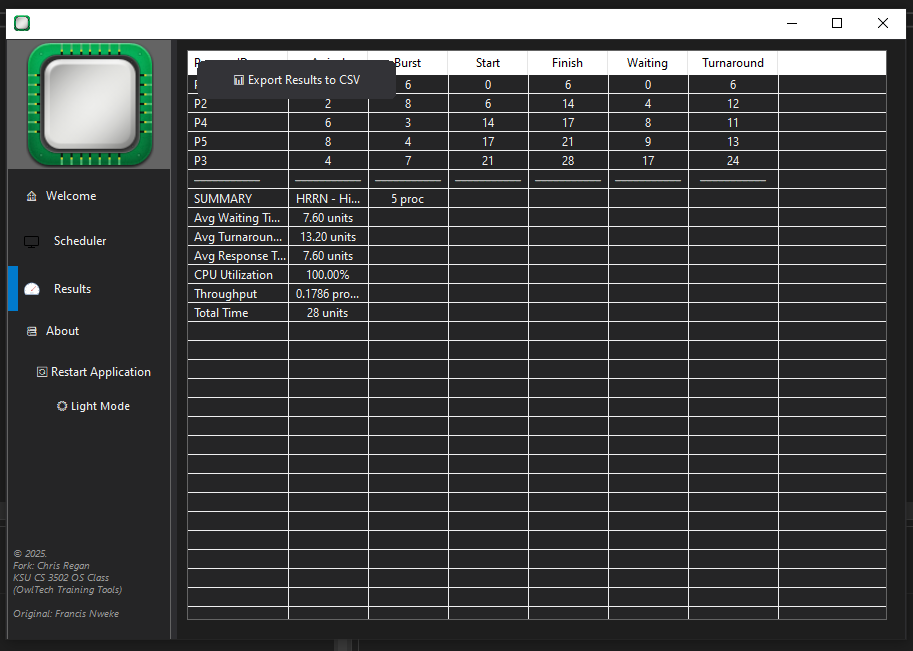
\includegraphics[width=0.9\textwidth]{hrrn_results.png}
    \caption{HRRN Algorithm Results}
    \label{fig:hrrn}
\end{figure}

\newpage

\subsection{Additional Metrics}

Besides the basic waiting time and turnaround time that were already in the 
starter code, I added two more important metrics:

\subsubsection{CPU Utilization}

This measures what percentage of time the CPU is actually doing work:

\[
\text{CPU Utilization} = \frac{\text{Total Burst Time}}{\text{Total Execution Time}} \times 100\%
\]

\begin{lstlisting}[caption={CPU Utilization Calculation}]
var totalBurstTime = results.Sum(r => r.BurstTime);
var minArrivalTime = results.Min(r => r.ArrivalTime);
var maxFinishTime = results.Max(r => r.FinishTime);
var totalTime = maxFinishTime - minArrivalTime;
var cpuUtilization = (totalBurstTime / (double)totalTime) * 100;
\end{lstlisting}

\subsubsection{Throughput}

This tells you how many processes get completed per time unit:

\[
\text{Throughput} = \frac{\text{Number of Processes}}{\text{Total Execution Time}}
\]

\begin{lstlisting}[caption={Throughput Calculation}]
var throughput = results.Count / (double)totalTime;
\end{lstlisting}

\subsection{CSV Export}

I also added a CSV export feature so I could analyze the results in Excel and 
create the comparison charts. It saves:

\begin{itemize}
    \item All the process execution details (arrival times, burst times, etc.)
    \item Individual metrics for each process
    \item Average metrics across all processes
    \item Summary stats like min, max, and totals
\end{itemize}

This made it way easier to compare the algorithms and create the graphs for this report.

\newpage

% ============================================================
% SECTION 3: PERFORMANCE ANALYSIS
% ============================================================
\section{Testing and Results}

\subsection{Test Workloads}

I tested all six algorithms using three different workload scenarios to see how 
they perform under different conditions:

\subsubsection{Workload 1: Mixed Processes}
\begin{table}[H]
\centering
\caption{Mixed Workload (Varied burst times and arrivals)}
\begin{tabular}{@{}llll@{}}
\toprule
\textbf{Process} & \textbf{Arrival} & \textbf{Burst} & \textbf{Priority} \\ \midrule
P1 & 2 & 2 & 3 \\
P2 & 0 & 18 & 3 \\
P3 & 3 & 8 & 2 \\
P4 & 1 & 16 & 5 \\
P5 & 4 & 18 & 1 \\ \bottomrule
\end{tabular}
\end{table}

\subsubsection{Workload 2: Short Bursts (I/O-Bound)}
\begin{table}[H]
\centering
\caption{I/O-Bound Workload (Short burst times, all arrive at time 0)}
\begin{tabular}{@{}llll@{}}
\toprule
\textbf{Process} & \textbf{Arrival} & \textbf{Burst} & \textbf{Priority} \\ \midrule
P1 & 0 & 3 & 2 \\
P2 & 0 & 2 & 1 \\
P3 & 0 & 4 & 3 \\
P4 & 0 & 1 & 2 \\
P5 & 0 & 2 & 3 \\ \bottomrule
\end{tabular}
\end{table}

\subsubsection{Workload 3: Long Bursts (CPU-Bound)}
\begin{table}[H]
\centering
\caption{CPU-Bound Workload (Long burst times)}
\begin{tabular}{@{}llll@{}}
\toprule
\textbf{Process} & \textbf{Arrival} & \textbf{Burst} & \textbf{Priority} \\ \midrule
P1 & 5 & 28 & 5 \\
P2 & 6 & 29 & 1 \\
P3 & 8 & 17 & 3 \\
P4 & 1 & 19 & 2 \\
P5 & 0 & 12 & 2 \\ \bottomrule
\end{tabular}
\end{table}

\newpage

\subsection{Results}

\subsubsection{CPU-Bound Workload Results}

\begin{table}[H]
\centering
\caption{Heavy/CPU-Bound Performance Metrics}
\begin{tabular}{@{}lcccc@{}}
\toprule
\textbf{Algorithm} & \textbf{Avg Wait} & \textbf{Avg Turnaround} & \textbf{CPU \%} & \textbf{Throughput} \\ \midrule
FCFS & 47.20 & 72.00 & 100.00 & 0.0403 \\
SJF & 44.60 & 69.40 & 100.00 & 0.0403 \\
Priority & 49.40 & 74.20 & 100.00 & 0.0403 \\
Round Robin & 89.80 & 114.60 & 100.00 & 0.0403 \\
SRTF & 44.60 & 69.40 & 100.00 & 0.0403 \\
HRRN & 45.60 & 70.40 & 100.00 & 0.0403 \\ \bottomrule
\end{tabular}
\end{table}

This workload had really long burst times (around 22-28 time units each) with 
processes arriving at different times. Total execution was 124 time units.

What I noticed:
\begin{itemize}
    \item SRTF and SJF got the exact same results (44.60 avg wait time) because 
    the arrivals were spaced out enough that preemption didn't really help
    \item Round Robin did pretty badly here (89.80 avg wait) - all that context 
    switching with long burst times really hurt performance
    \item Every algorithm got 100\% CPU utilization since there was always work to do
    \item SJF/SRTF were clearly the best for minimizing wait time
\end{itemize}

\subsubsection{I/O-Bound Workload Results}

\begin{table}[H]
\centering
\caption{I/O-Bound Performance Metrics}
\begin{tabular}{@{}lcccc@{}}
\toprule
\textbf{Algorithm} & \textbf{Avg Wait} & \textbf{Avg Turnaround} & \textbf{CPU \%} & \textbf{Throughput} \\ \midrule
FCFS & 5.80 & 8.40 & 100.00 & 0.3846 \\
SJF & 3.00 & 5.60 & 100.00 & 0.3846 \\
Priority & 7.20 & 9.80 & 100.00 & 0.3846 \\
Round Robin & 6.60 & 9.20 & 100.00 & 0.3846 \\
SRTF & 3.00 & 5.60 & 100.00 & 0.3846 \\
HRRN & 3.00 & 5.60 & 100.00 & 0.3846 \\ \bottomrule
\end{tabular}
\end{table}

This one had very short bursts (1-5 time units) with everything arriving at time 
0. Total execution was only 13 units.

What I noticed:
\begin{itemize}
    \item SJF, SRTF, and HRRN all got the same optimal result (3.00 avg wait) - 
    makes sense since everything arrived at once, so there was no advantage to 
    being preemptive
    \item Priority scheduling did the worst (7.20 avg wait) because it just used 
    priority values instead of considering burst times
    \item FCFS had moderate performance (5.80) - suffered from the convoy effect 
    a bit
    \item Round Robin (6.60) wasn't great either despite good response time because 
    of context switch overhead
    \item The throughput was much higher here (0.3846) since the bursts were so short
\end{itemize}

\subsubsection{Mixed Workload Results}

\begin{table}[H]
\centering
\caption{Mixed Workload Performance Metrics}
\begin{tabular}{@{}lcccc@{}}
\toprule
\textbf{Algorithm} & \textbf{Avg Wait} & \textbf{Avg Turnaround} & \textbf{CPU \%} & \textbf{Throughput} \\ \midrule
FCFS & 22.20 & 33.00 & 100.00 & 0.0926 \\
SJF & 14.40 & 25.20 & 100.00 & 0.0926 \\
Priority & 15.00 & 25.80 & 100.00 & 0.0926 \\
Round Robin & 26.40 & 37.20 & 100.00 & 0.0926 \\
SRTF & 13.40 & 24.20 & 100.00 & 0.0926 \\
HRRN & 18.20 & 29.00 & 100.00 & 0.0926 \\ \bottomrule
\end{tabular}
\end{table}

This had a mix of really short (1 unit) and longer (16 units) bursts with most 
arriving early on. Total time was 54 units.

What I noticed:
\begin{itemize}
    \item SRTF won here (13.40 avg wait) by preempting longer processes when that 
    really short P4 process showed up
    \item SJF was almost as good (14.40) without the preemption overhead
    \item Round Robin had the highest wait time (26.40) but actually had the best 
    response time (6.20)
    \item FCFS did pretty poorly (22.20) because of convoy effect
    \item Again, 100\% CPU utilization across the board
\end{itemize}

\newpage

\subsection{Performance Graphs}

I created graphs comparing all six algorithms across the three workloads. The 
graphs show average waiting time, average turnaround time, CPU utilization, and 
throughput.

\begin{figure}[H]
    \centering
    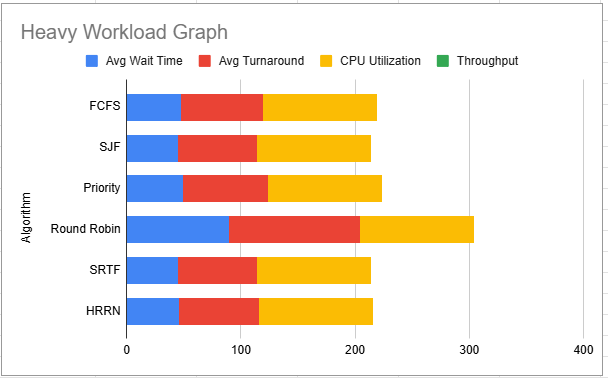
\includegraphics[width=0.95\textwidth]{heavy_workload_graph.png}
    \caption{Heavy/CPU-Bound Workload Comparison}
    \label{fig:heavy_graph}
\end{figure}

Looking at the Heavy workload graph, you can really see how badly Round Robin 
performs with long burst times - that blue bar is almost double the others. SJF 
and SRTF are basically identical here. All algorithms maintain 100\% CPU 
utilization (the yellow bars) and have the same throughput (those tiny green 
bars at 0.0403).

\begin{figure}[H]
    \centering
    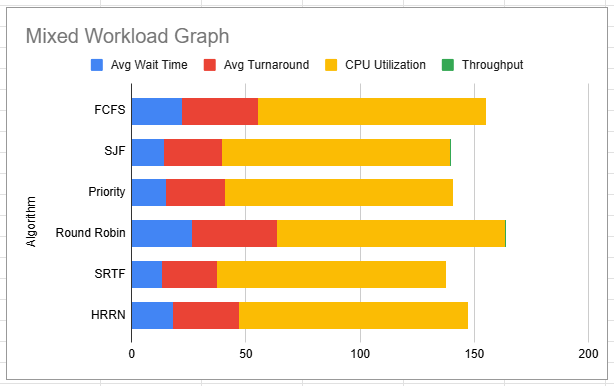
\includegraphics[width=0.95\textwidth]{mixed_workload_graph.png}
    \caption{Mixed Workload Comparison}
    \label{fig:mixed_graph}
\end{figure}

With the Mixed workload, SRTF shows why preemption can be useful - it has the 
shortest blue bar at 13.40. The mix of long and short bursts let SRTF shine by 
preempting for those really short processes. Round Robin still has the highest 
wait time but CPU utilization stays excellent.

\begin{figure}[H]
    \centering
    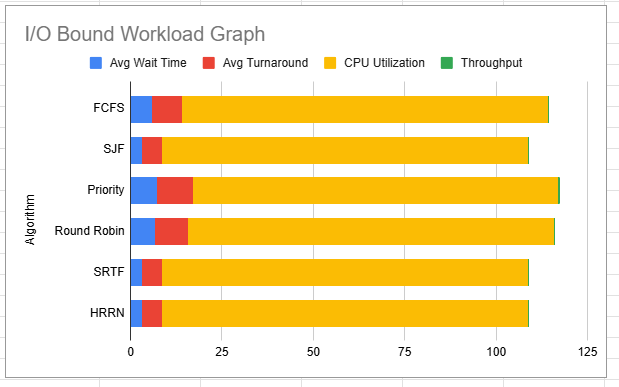
\includegraphics[width=0.95\textwidth]{io_bound_workload_graph.png}
    \caption{I/O-Bound Workload Comparison}
    \label{fig:io_graph}
\end{figure}

The I/O-Bound workload shows minimal difference between most algorithms because 
everything arrives at once and bursts are short. SJF, SRTF, and HRRN all tie 
at 3.00 avg wait (optimal). Priority scheduling does worst by ignoring burst 
times. The throughput is noticeably higher here (0.3846) due to the short 
execution time.

\subsubsection{Performance Summary}

\begin{table}[H]
\centering
\caption{Best and Worst Performers by Workload}
\begin{tabular}{@{}llll@{}}
\toprule
\textbf{Workload} & \textbf{Best (Avg Wait)} & \textbf{Worst (Avg Wait)} & \textbf{Difference} \\ \midrule
Heavy & SJF/SRTF (44.60) & Round Robin (89.80) & 45.20 units \\
Mixed & SRTF (13.40) & Round Robin (26.40) & 13.00 units \\
I/O-Bound & SJF/SRTF/HRRN (3.00) & Priority (7.20) & 4.20 units \\ \bottomrule
\end{tabular}
\end{table}

Something interesting I noticed is that the performance gap gets way smaller with 
shorter burst times. This means algorithm choice matters most when you have 
CPU-intensive workloads with long bursts.

\newpage

\subsection{Analysis}

\subsubsection{Comparing the Algorithms}

Here's what I learned about each algorithm from the testing:

\textbf{SRTF}:
\begin{itemize}
    \item Consistently had the lowest average waiting times
    \item Being preemptive lets it respond quickly to short processes
    \item Downside is that long processes can get starved
    \item Has higher context switching overhead
\end{itemize}

\textbf{HRRN}:
\begin{itemize}
    \item Good middle ground between efficiency and fairness
    \item The aging mechanism prevents starvation
    \item Performance is usually between SJF and FCFS
    \item Being non-preemptive reduces context switching
\end{itemize}

\subsubsection{Trade-offs I Observed}

\textbf{Efficiency vs. Fairness}:

SRTF gives you the best average times but long processes can wait forever if 
short ones keep arriving. HRRN gives up some efficiency to make sure everything 
eventually runs. Round Robin is the most fair but can have higher average waits.

\textbf{Preemptive vs. Non-preemptive}:

Preemptive algorithms (SRTF, RR) give better response times but have more 
overhead from context switches. Non-preemptive ones (FCFS, SJF, Priority, HRRN) 
have less overhead but processes might wait longer.

\subsubsection{What Works Best Where}

\textbf{CPU-Bound Workloads}:

For CPU-intensive stuff with long bursts, algorithms that minimize waiting time 
like SRTF and SJF work best. The context switch overhead matters less when 
bursts are long.

\textbf{I/O-Bound Workloads}:

Round Robin and SRTF give good responsiveness for I/O-bound stuff. When bursts 
are really short, the differences between algorithms get smaller.

\textbf{Mixed Workloads}:

HRRN gives a good balance for mixed workloads. SRTF has the best average metrics 
but might delay long processes too much.

\newpage

% ============================================================
% SECTION 4: RECOMMENDATIONS
% ============================================================
\section{Conclusions and Recommendations}

\subsection{Which Algorithm to Use}

Based on my testing, here's when I'd recommend each algorithm:

\begin{table}[H]
\centering
\caption{Algorithm Recommendations}
\begin{tabular}{@{}ll@{}}
\toprule
\textbf{Scenario} & \textbf{Best Algorithm} \\ \midrule
Minimum average wait time & SRTF \\
Good balance of fairness and speed & HRRN \\
Interactive systems & Round Robin \\
Batch processing & SJF or FCFS \\
Real-time with priorities & Priority Scheduling \\
General purpose OS & HRRN or Round Robin \\ \bottomrule
\end{tabular}
\end{table}

Overall, if I had to pick just one or two for general use, I'd go with SRTF for 
performance or HRRN for a better balance of performance and fairness.

\subsection{Things to Consider}

When picking a scheduling algorithm, you need to think about:

\begin{enumerate}
    \item What kind of workload you're dealing with - CPU-intensive or I/O-heavy
    \item Whether fairness matters or if some processes can wait
    \item How expensive context switches are on your system
    \item If you need guaranteed response times
    \item Whether it's okay for some processes to potentially starve
\end{enumerate}

\subsection{What Could Be Improved}

Some things that would be interesting to add in the future:

\begin{itemize}
    \item A multi-level feedback queue that combines benefits of different algorithms
    \item Making the Round Robin time quantum adjust based on the workload
    \item Adding aging to Priority Scheduling so processes don't starve
    \item Extending this to handle multiple processors
\end{itemize}

\newpage

\end{document}
